\onecolumn

\begin{titlepage}
\null
\vspace{15mm}

\begin{flushleft}
\begin{bfseries}
	\vskip2mm
	\Huge{Design Document for\\ Better Graphics For A Robotics Grasping GUI}\\
	\vspace{15mm}
	\textbf{\huge Shady Robots} \\
	\vskip2mm
	\large{Group 12}
	\vskip5mm
	\Large{Justin Bibler \\
	Matthew Huang \\
	Daniel Goh \\}
\end{bfseries}

\vspace{15mm}
\Large{CS461: Senior Software Engineering Project} \\
\Large{Fall 2016} \\

\vspace{5mm}

\today

\vfill

\begin{normalsize}
{\bf Abstract:}
Our customer is using a simulation to create visuals that are used for online data collection.
This simulation is using outdated libraries which result in outdated graphics.
Design definitions outlined in this document will be used to accomplish our customer's request.
The request being to update the simulation's graphics with warm cool shaders, shadows and silhouettes.

{\bf Keywords:} OpenInventor, OpenGL, OpenRave, shaders, warm cool shaders, silhouettes, shadows, robotic simulation, geometry, visualization, render, vertex lines
\end{normalsize}
\end{flushleft}

\newpage

\end{titlepage}

\subsection{Introduction}
\begin{flushleft}

\subsubsection{Purpose}
The purpose of this document is to elaborate on the design and logic of how we will be implementing our requirements.

\subsubsection{Scope}
The scope of this document is solely about how new features will be implemented and how those implementations will be tested.

\subsubsection{Context}
Currently, our client is using visualizations, of a robot hand grasping objects, to collect data online.
These visualizations are created from a simulation program (OpenRave); the data collected is used to create a model of the human grasp.
However, the current graphics in the simulation are outdated.
It is hard to see and understand the shapes and contact points represented in the scene.

The context of this document is focused primarily on the visuals of the project.

\subsubsection{Summary}
In clauses 3 to 5, Matthew Huang outlines the design of Gooch shading, silhouettes, and run-time analysis with CodeXL respectively.
In clauses 6 to 8, Justin Bibler outlines the design of shadow volumes, performance benchmarks using FRAPS \cite{fraps}, and methods of code maintainability.
In clauses 9 and 10, Daniel Goh outlines the methods and guidelines to create the online survey, and methods to analyze and visualize the collected data.

\newpage

% References
\bibliographystyle{IEEEtran}
\bibliography{designdoc}

\subsection{Glossary}

FRAPS - FRAPS is a benchmarking, screen capture and screen recording utility for Windows.

FPS - Frames per second (FPS) is a unit that measures display device performance.

Frequency (statistics) - Frequency of a particular data value is the number of times the data value occurs. \cite{freq}

\newpage

% Matt's Section
\subsection{Requirement: Gooch Shading}
\large{By Matthew Huang}

\normalsize
\subsubsection{Design Concerns}
Our team is assuming that the rendering for the 3D scene is done by OpenRave and not the Qt GUI.
The OpenGL Shading Language (GLSL) will be used to implement Gooch Shading. 
Gooch Shading requires use of both the vertex buffer and fragment buffer.
In its implementation, Gooch Shading makes use of a warm and cool color to highlight its objects.
Gooch shaded objects should not have any "blacked out" areas on them.

\subsubsection{Design Stakeholders}
Cindy Grimm, Justin Bibler, Matthew Huang, and Daniel Goh

\subsubsection{Context Viewpoint}

\begin{figure} [H]
  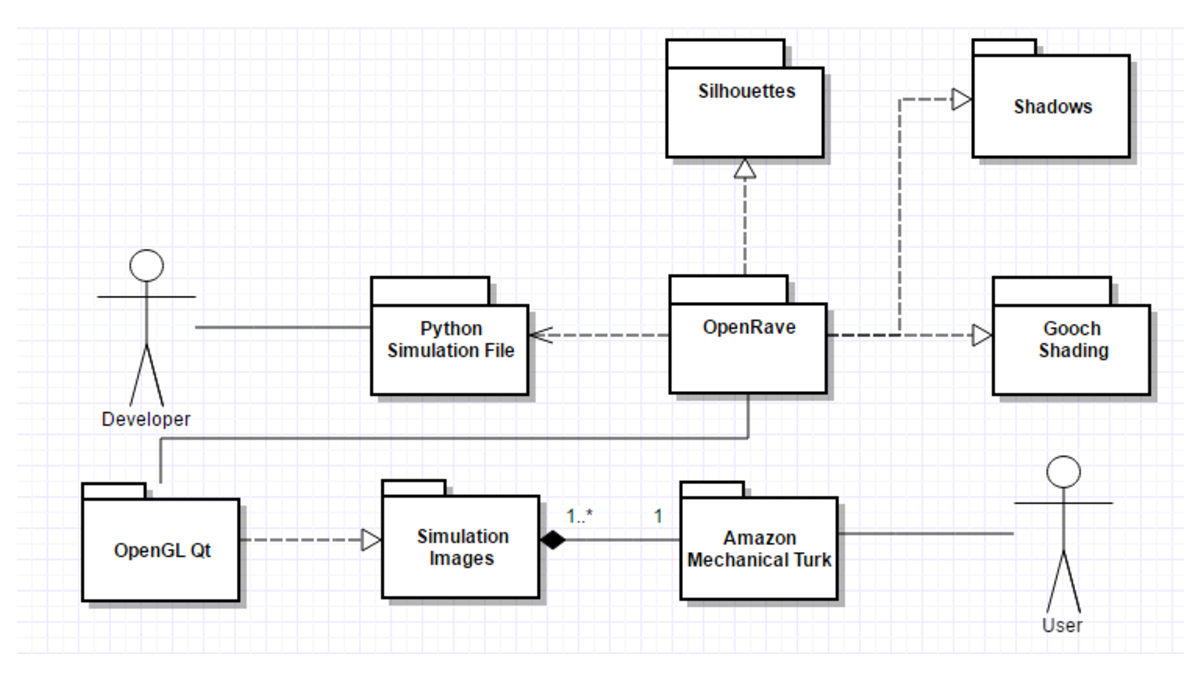
\includegraphics[scale=0.8]{designdoc_v1/Gooch_Shading_context.eps}
  \caption
{ \newline \hspace{\linewidth}
Context Viewpoint Diagram that shows relation of Gooch Shading to OpenRave}
  \label{fig:Gooch_Shading_context}
\end{figure}

\paragraph{Design View}
Gooch Shading will be implemented into OpenRave assuming that OpenRave is indeed the renderer.
A successful Gooch Shading implementation will use warm and cool coloring to help improve object geometry (which will be displayed by Qt).
Improved object geometry means improved simulation images for users of the Amazon Mechanical Turk.
The updated images will aid user confidence in how they answer the mechanical turk questions which will improve the data collected.

\subsubsection{Compositional Viewpoint}

\begin{figure} [H]
  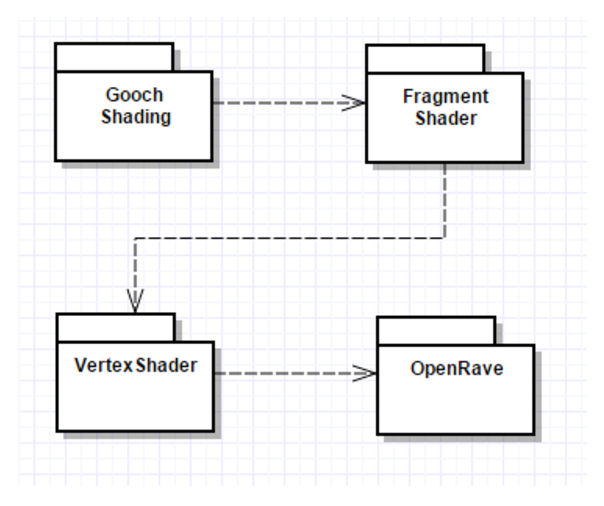
\includegraphics[scale=0.9]{designdoc_v1/Gooch_Shading2_composition.eps}
  \caption
{ \newline \hspace{\linewidth}
Compositional Viewpoint Diagram that shows the flow of Gooch Shading implementation to OpenRave}
  \label{fig:Gooch_Shading2_composition}
\end{figure}

\paragraph{Design View}
This implementation of Gooch Shading makes use of the following entities: the vertex buffer, the fragment buffer, and the renderer (OpenRave). 
OpenRave will supply relevant variables (camera position, object position, light position, colors, etc.) to the vertex shader.
The vertex shader calculates the light position and passes its variables to the fragment shader.
The fragment shader is the entity that shades the 3D objects.
In it, it calculates the diffuse lighting along with the augmented warm and cool colors that will shade the object.
The augmented warm and cool colors are determined by the object's original color and the Gooch Shading weight.
After that, linear interpolation is done on the two augmented colors to determine what the final color will be for that fragment.
In GLSL, linear interpolation can be done using the mix() function.
This shading will highlight the entire object leaving no completely "blacked out" areas.

\newpage

\subsubsection{Logical Viewpoint}

\begin{figure} [H]
  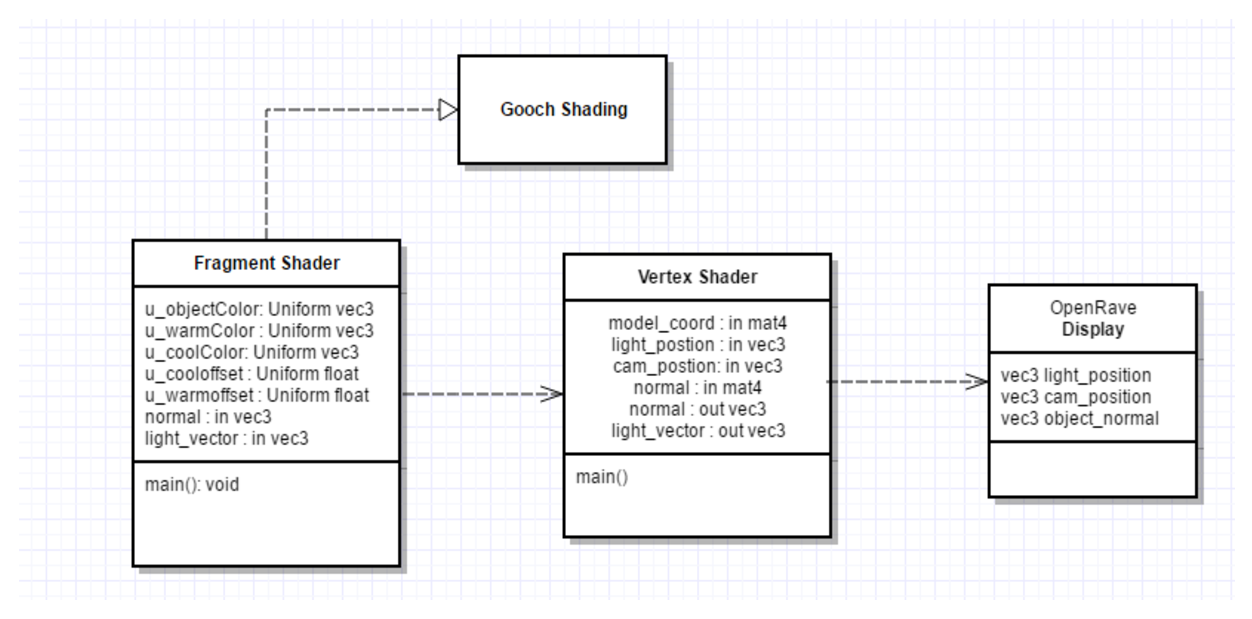
\includegraphics[scale=0.8]{designdoc_v1/Gooch_Shading_composition.eps}
  \caption
{ \newline \hspace{\linewidth}
Logical Viewpoint Diagram that shows the implementations of Gooch Shading}
  \label{fig:Gooch_Shading_composition}
\end{figure}

\paragraph{Design View}
In the code, the Gooch Shading inputs will come from the display function of the renderer.
The display function obviously holds many variables, but will only pass the following variables to the vertex shader:
\begin{itemize}
\item Camera position.
\item Object normal vector.
\item Light position.
\item Object position (model coordinates).
\item Colors (warm, cool, object original).
\end{itemize}

The warm and cool colors are determined by the developer and the object color is supplied by the python file passed into OpenRave.
The camera and object position are needed to determine the object's world coordinates (which is done in the vertex shader).
All these variables are written in GLSL.
GLSL can be used if the version of OpenGL on the system is 2.0 or above; the current version on the system will be updated to meet this requirement.
The vertex shader calculates the light vector using the object's world coordinates and the light position. 
Afterwards, it outputs the colors (warm, cool, object), the light vector, and the object's normal vector to the fragment shader.
The fragment shader will then determine the diffuse lighting for the object (diffuse lighting is the dot product of the object's normal vector with the light vector).
Following that, it augments the warm and cool colors (using the formula: color + object\_color*gooch\_shading\_weight), and then linearly interpolates between them using the GLSL mix() function \cite{glslmix}.
This interpolation determines the shade coloring for that specific fragment of the object.

\newpage

\subsection{Requirement: Silhouettes}
\large{By Matthew Huang}

\normalsize
\subsubsection{Design Concerns}
Silhouettes need to give the 3D shapes in the simulation solid borders so that the objects in the scene can be differentiated from each other.
The silhouettes need to be working in situations where objects overlap with each other and under multiple viewpoints. 
The algorithm for how the silhouettes are drawn needs to be clear.

\subsubsection{Design Stakeholders}
Cindy Grimm, Justin Bibler, Matthew Huang, and Daniel Goh

\subsubsection{Context Viewpoint}

\begin{figure} [H]
  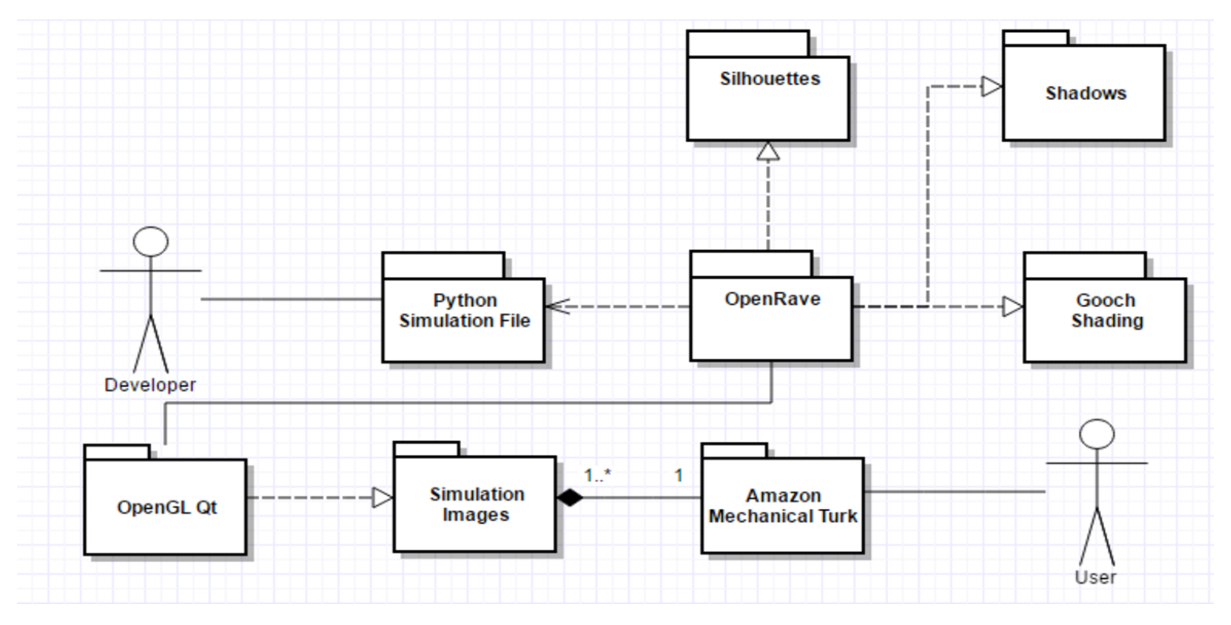
\includegraphics[scale=0.8]{designdoc_v1/Silhouettes_context.eps}
  \caption
{ \newline \hspace{\linewidth}
Context Viewpoint Diagram that that shows relation of silhouettes to OpenRave}
  \label{fig:Silhouettes_context}
\end{figure}

\paragraph{Design View}
The context viewpoint for silhouettes is essentially the same as the one for shaders.
That is to say, its end goal is to improve the end user experience by enhancing the images sent to the Amazon Mechanical Turk.
Additionally, it will also be implemented in OpenRave.
Where it differs, however, is in how it affects the simulation images.
Instead of highlighting 3D object geometry like the Gooch Shading will do, silhouettes will emphasize an object's borders (I.E. where an object begins and ends).
These silhouettes are meant to help users differentiate between objects in the simulation images.

\subsubsection{Compositional Viewpoint}

\begin{figure} [H]
  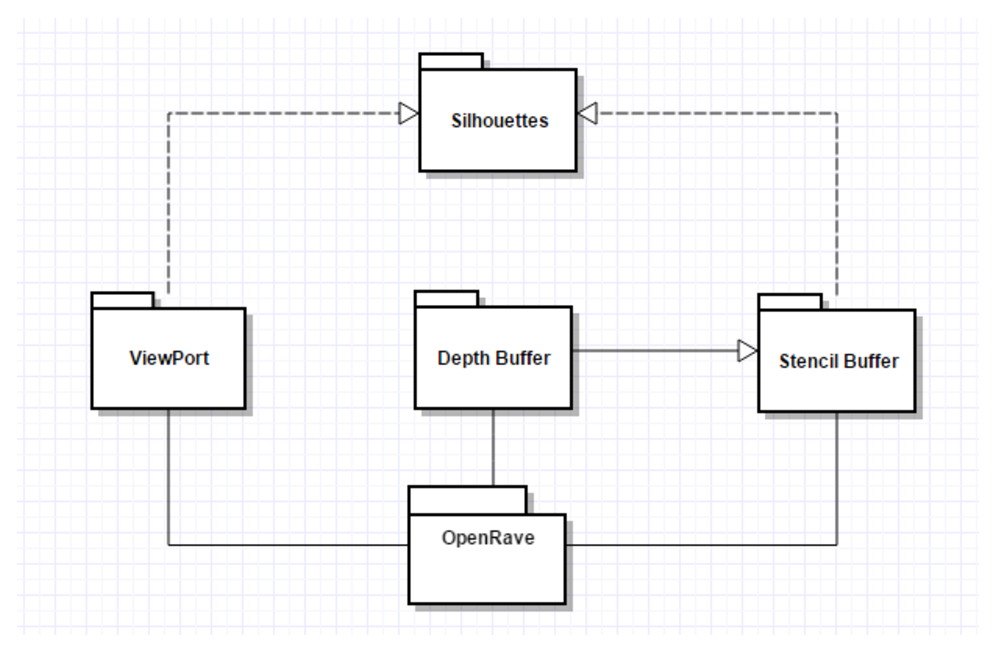
\includegraphics[scale=0.9]{designdoc_v1/Silhouettes_composition.eps}
  \caption
{ \newline \hspace{\linewidth}
Compositional Viewpoint Diagram that show relationship of Silhouettes}
  \label{fig:Silhouettes_composition}
\end{figure}

\paragraph{Design View}
Silhouettes will be implemented using a combination of the Stencil Buffer along with manipulation of the view port.
The Stencil Buffer is an optional extension of the depth buffer; both of them can be enabled in OpenRave using the glEnable() function (I.E. glEnable(GL\_STENCIL\_TEST) \cite{depthstencils}.
The Stencil Buffer gives you control over which fragments of the object should be drawn and which shouldn’t.
The viewport allows you to translate your objects in windows coordinates (I.E. pixels).
The basic algorithm to implement these silhouettes is to move the object in one direction (x, y, -x, or -y), draw the object with the stencil buffer enabled, and then repeat until you have drawn in all four directions.
The amount you move the object will affect how large of a silhouette is made.
To draw a solid color silhouette (I.E. black), draw the silhouette using a solid color version of the object.
Additionally, because the stencil buffer gives you control over what fragments of the object are drawn, overlapping objects are dealt with easily.

\newpage

\subsubsection{Algorithm Viewpoint}
Silhouette Algorithm pseudo-code implementation

\begin{lstlisting}
glEnable(stencil buffer)
glDisable(depth buffer)
glDisable(color buffer)
Clear(stencil buffer)
glStencilFunc(Always Pass)	//tell the stencil buffer to let all fragments pass
glStencilOp(Increment)		//tell stencil buffer to increment on acceptance
glViewPort(Move +y)	//Move object by some amount of pixels in the y direction
Display(object)		//render object
glViewport(Move -y)
Display(object)
glViewport(Move +x, +y)
Display(objecT)
glViewport(Move -x)
Display(object)
glViewport(Move +x)
glEnable(color buffer)
glEnable(depth buffer)
glStencilFunc(Pass if value is 2 or 3)
\end{lstlisting}

\paragraph{Design View}
The pseudo-code created above was based off of the algorithm available on the opengl silhouette edges webpage \cite{siledges}.
In general, the algorithm is easily to follow if you know how to manipulate the stencil buffer and the view port (which we do).
To summarize, glViewport() is the function that will be translating the object in windows coordinates (I.E. pixels), glStencilFunc() is the function that gives the developer control over which fragments to render, and glStencilOp gives the developer control over what happens to the stencil value of the fragment if it's accepted.
The Display() function will presumably be somewhere in OpenRave and will be the function that ultimately renders the object.
Importantly note that in total, Display() is called four times in the algorithm meaning that the object must be rendered four times to create the silhouette.
If this factor affects the runtime of the system to the point where performance benchmarks are not met, the algorithm should be changed.

\newpage

\subsection{Requirement: Creation of Online Survey}
\large{By Matthew Huang}

\normalsize
\subsubsection{Design Concerns}
The modifications made to the current OpenRave system (Gooch Shading, silhouettes, and shadows) may slow the system down.
As a requirement, the modified system must run at a minimum 30 frames per second (fps).
As a requirement, the modified system must render the initial simulation image within 30 seconds.
To assist with these requirements, the debugger shall have the ability to track function calls.

\subsubsection{Design Stakeholders}
Cindy Grimm, Justin Bibler, Matthew Huang, and Daniel Goh

\subsubsection{Context Viewpoint}

\begin{figure} [H]
  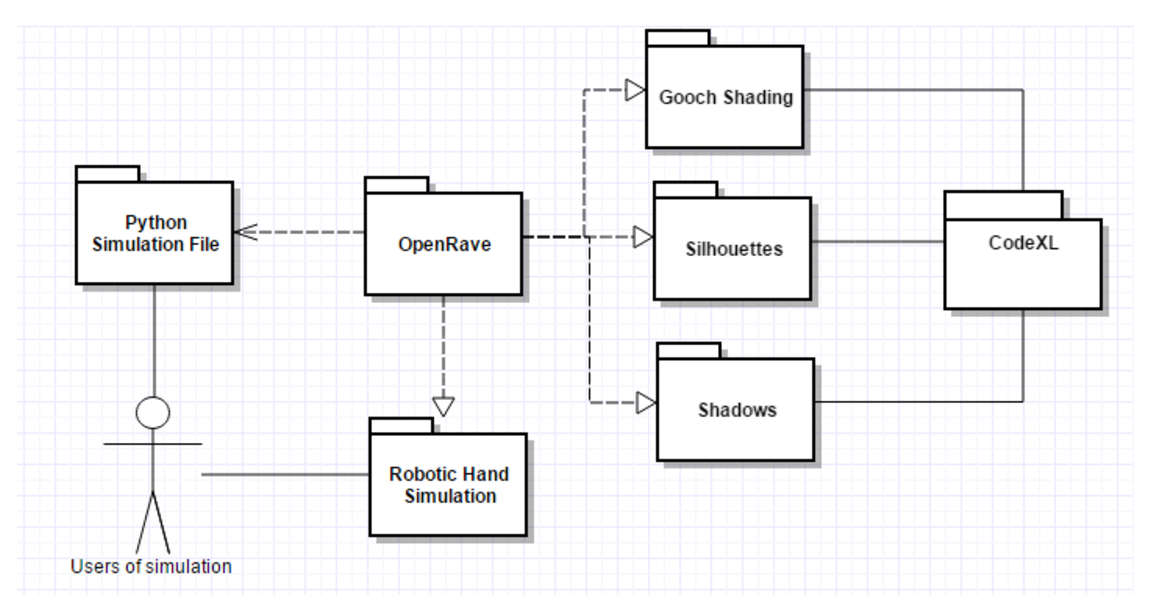
\includegraphics[scale=0.9]{designdoc_v1/CodeXL_Context.eps}
  \caption
{ \newline \hspace{\linewidth}
Context Viewpoint Diagram that shows relationship of CodeXL}
  \label{fig:CodeXL_Context}
\end{figure}

\paragraph{Design View}
CodeXL will be primarily used to track our Gooch Shading, silhouette, and shadow implementations.
Its main goal is to monitor the effect that these three implementation have on the OpenRave simulation.
If the implementations cause the robotic hand simulation to drop below 30 frames per second, CodeXL should be able to pinpoint where the cause originated from.
The goal of this is to ensure a pleasant and smooth experience for the users of the robotic hand simulation.

\subsubsection{Dependancy Viewpoint}

\begin{figure} [H]
  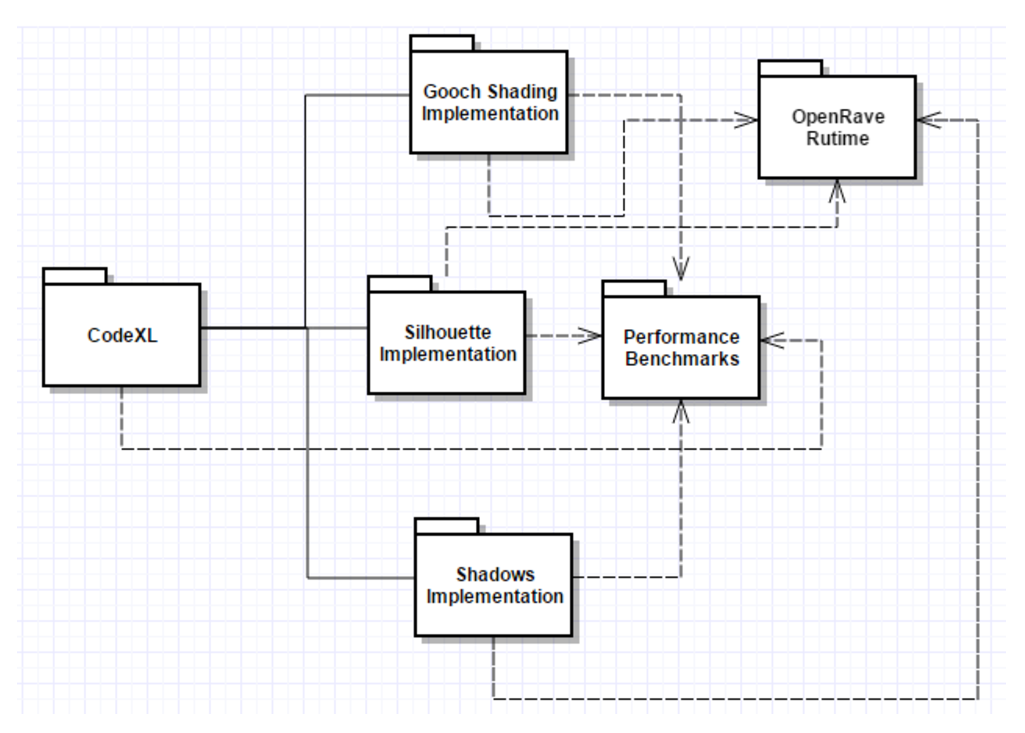
\includegraphics[scale=0.9]{designdoc_v1/CodeXL_Dependency.eps}
  \caption
{ \newline \hspace{\linewidth}
Dependancy Viewpoint Diagram that shows dependencies of CodeXL}
  \label{fig:CodeXL_Dependency}
\end{figure}

\paragraph{Design View}
How CodeXL monitors the three implementations will depend on the performance benchmarks for the whole system.
If the implementations are in and the performance benchmarks are met, inefficient function calls or other issues brought up by CodeXL may be ignored.
If the implementations bring the system down below performance benchmarks, CodeXL will have to display what is happening in the system that is causing it to slow down.
Causes like large amounts of the same function calls, long running functions, and other bugs should be tracked.
Specifically, if the frames drop below 30fps, CodeXL should be able track which implementation (or which combination of implementations) is causing the most performance loss.
If the silhouettes are causing significant performance loss, they will be the first to be refactored since there are many ways to implement silhouettes. 
Gooch Shading is less flexible in its implementation so refactoring it will have a lower priority (shadows is somewhere between silhouettes and Gooch Shading).

If OpenRave takes more than 30 seconds to render, problems likely exist in how we initialize our scene.
In this situation, CodeXL will be used to primarily track activity in the Display function since that is the function the renders the initial scene.
Other object initialization functions will not be tracked since we assume that they are pulled from libraries we have no control over.
Additionally, performance benchmarks will only be changed as a last resort (I.E. we cannot refactor our implementations anymore).

\subsubsection{Interface Viewpoint}

\begin{figure} [H]
  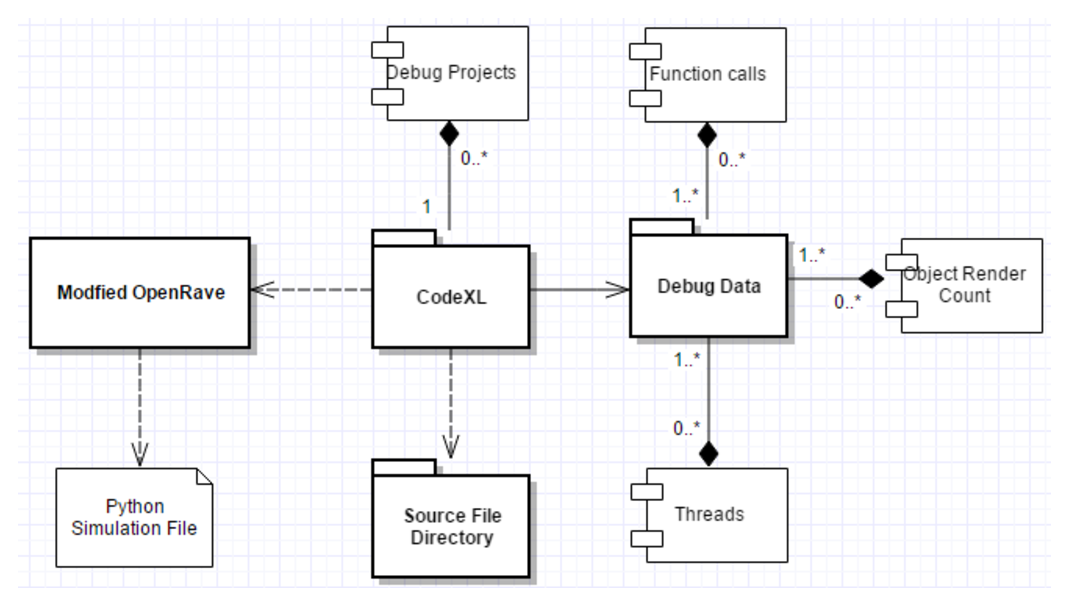
\includegraphics[scale=0.9]{designdoc_v1/CodeXL_Interface.eps}
  \caption
{ \newline \hspace{\linewidth}
Interface Viewpoint Diagram that shows the interface relations of CodeXL}
  \label{fig:CodeXL_Interface}
\end{figure}

\paragraph{Design View}
To monitor OpenRave, create a debug project in CodeXL and set the OpenRave executable as the debug project's executable.
Additionally, provide the python simulation file as a command line argument and set the source file directory to where the python file lives (this is all done in creating the debug project).
Afterwards, execute the debug project and CodeXL will display debug information such as rendered objects, created threads, and function calls (if you turn that on).
Note, however, that tracking function calls slows down CodeXL significantly so it shouldn't be used for basic testing.
Past that, CodeXL also provides access to the source code currently running directly on the CodeXL GUI.

\newpage

%Justin's section
\subsection{Requirement: Shadows}
\large{By Justin Bibler}

\normalsize
\subsubsection{Software Design Description}
Our client requires us to add shadows into the simulation's graphics.
The addition of shadows will improve the overall graphics of the simulation, which will help a user better understand where an object is within a 3D space.

\subsubsection{Design Stakeholders}
Justin Bibler, Matthew Huang, and Daniel Goh

\subsubsection{Design Concerns}
All stakeholder share similar design concerns.

Shadows design concerns:
\begin{enumerate}
\item Will our shadow implementations have a major impact on FPS.
\item Will our shadows be too pixelated.
\item Will users be able to better understand where an object is because of our shadow implementation.
\end{enumerate}

\newpage

\subsubsection{Design Views}
\paragraph{Interface Design}
This section is dedicated to talking about the graphical quality of our shadow implementation.

\subparagraph{Design Concerns}
Interface design concerns:
\begin{enumerate}
\item Will users be able to better understand where an object is because of our shadow implementations.
\item Will our shadows be too pixelated.
\end{enumerate}

\subparagraph{Design Elements}
\textbf{Name}
Shadow Interface.

\textbf{Type}
Visual, or Graphic.

\textbf{Purpose}
Shadows with the simulation exist to better help users understand an objects location within a 3D space.

\textbf{Relationship}
The quality of the visuals rely heavily on the design discussed later within the Algorithmic implementation of shadows.

\textbf{Interface attribute}
Depending on the implementation in the algorithm viewpoint, every 3D model within the simulation should have a shadow.
Whether or not the shadow is visible is dependent on if there is a surface that the shadow volume collides with.
These shadows should have minimal pixelation.
In addition, the shadows should be relatively close in shape to their original models, as to not confuse what shadow is projected out from what object.
All of this is done so that the users will easily be able to understand what shadow is related to what object, and to receive a better understanding of the 3D environment in the simulation.

\newpage

\paragraph{Algorithm Viewpoint}
The idea of the shadow volume algorithm is to extend the silhouettes of objects that are in contact with light sources into volumes.
And whenever another object falls within the shadow objects volume, it is rendered in a different way. \cite{shadow}

\subparagraph{Design Concerns}
Algorithm design concerns:
\begin{enumerate}
\item Will the algorithm be costly to the simulation's FPS.
\end{enumerate}

\subparagraph{Design Elements}
\textbf{Name}
Algorithmic implementation of shadows.

\textbf{Type}
Algorithm, or method.

\textbf{Relationship}
Shaders, and the Shadow Interface.

\textbf{Design Constraints}
The implementation of shadows will most likely rely on the knowledge we gain from implementing warm cool shaders into the simulation.
That knowledge will allow us to better understand how the simulation is being rendered, making it easier for us to adjust and change certain shaders.
Another constraint that we have is that there is a relatively small amount of documentation related to OpenRave and OpenInventor.
This makes it difficult to find exactly where we need to implement shaders to get our desired results.

\textbf{Processing Attribute}
The bases of the algorithm will be using the depth fail test.
This will be done by first rendering all the objects in the scene into the depth buffer.
From here, we create shadow volumes for each object based on the objects silhouette projected into infinity relative to where the light is striking the object.
Then we render the volume into the stencil buffer based off the depth fail test.

Depth fail test:
\begin{enumerate}
\item If the depth test fails while rendering back facing polygons of the shadow volume, we increment the stencil buffer.
\item If the depth test fails while rendering the front facing polygons of the shadow volume, we decrement the stencil buffer.
\item Nothing happens if the test passes, or the stencil test fails.
\end{enumerate}

This depth fail test is conducted for each shadow volume.
Once the tests have concluded, the scene will be rendered into the viewport.
However, only the objects, or parts of objects, that have a stencil buffer value of zero will be rendered without alterations. \cite{shadow}

\newpage

\subsection{Requirement: Measuring the Simulation's FPS}
\large{By Justin Bibler}

\normalsize
\subsubsection{Software Design Description}
Our project requires us to measure and analyze the runtime and FPS of our altered simulation.
This is done so that we can ensure that our additions fulfill our performance metrics: the simulation must maintain an average 30 FPS.
 If we are unable to reach this metric our implementations will be considered incorrect, and will require revisions.

\subsubsection{Design Stakeholders}
Justin Bibler, Matthew Huang, and Daniel Goh

\subsubsection{Design Concerns}
All stakeholders share similar design concerns.

Requirement design concerns:
\begin{enumerate}
\item Failing to meet our target FPS and runtime will result in revisions of our implementations.
\item Will our measurements be accurate for the majority of computers.
\item Software used for measuring may cost money.
\end{enumerate}

\newpage

\subsubsection{Design Views}
\paragraph{Information Viewpoint}
The purpose of this viewpoint is describe how information will be gathered, and how it will be analyzed.
Our team will be using an external tool to obtain data related to the simulation's FPS.
 FRAPS will be used to examine the FPS and export the information into a file to be analyzed.

\subparagraph{Design Concern}
Interface viewpoint concerns:
\begin{enumerate}
\item FRAPS is paid software.
\item Will our measurements be accurate for the majority of computers.
\end{enumerate}

\subparagraph{Design Elements}
\subparagraph{Name}
Method of analyzing and collecting FPS data.

\textbf{Type}
Method.

\textbf{Purpose}
Data collected will be analyzed to ensure that our implementations into the simulation meet our requirements.

\textbf{Data attribute}
FRAPS will be used to capture data related to FPS, this will be done by using the benchmarking tools that come with the software.
We will run this test for one minute ten times, on five different sample simulations with our updated graphics.
This data will be exported into a file, from here we will analyze the data by finding the mean and median across all executions.
If these values are within a certain standard deviation of 30 FPS, our implementation will be considered correct.

\textbf{Author}
FRAPS is owned by Beepa.\cite{fraps}

\subsubsection{Rational}
Even though FRAPS is a paid software I've decided that it be best if we use it.
It's ability to export data into a file allows our group to easily obtain and analyze data.
Furthermore, our concern related to the validity of the data stems from the fact that our group members own above average computers.
Thus, testing on our computers would most likely be inaccurate relative to the average computer.
To circumvent this problem we plan to do most of our testing on the computers on the OSU campus.

\newpage

\subsection{Requirement: Code Maintainability}
\large{By Justin Bibler}

\normalsize
\subsubsection{Software Design Description}
The goal behind code maintainability is to increase the cost effectiveness of changes being made to a system. \cite{maintain}
Our group has made this a requirement because our client wishes to be able to easily change, or add into our implementations.
The primary logic behind this design is the use of good programming practices such as documentation, and commenting, but also the use of external resources which are described within the viewpoint below.

\subsubsection{Design Stakeholders}
Justin Bibler, Matthew Huang, and Daniel Goh

\subsubsection{Design Concerns}
All stakeholders share similar design concerns.

Requirement design concerns:
\begin{enumerate}
\item Cost of static code debugging tools.
\item Lack of documentation for preexisting code.
\item Lack of comments for preexisting code.
\end{enumerate}

\newpage

\subsubsection{Design Views}
\paragraph{Resource Viewpoint}
External resources will be used to help us maintain and upkeep our code quality.
The first resource we will be using, which within today's standard is almost a necessity, will be GitHub.
GitHub is a repository that is used for code version control.
Secondly, we will be using Cppcheck.
Cppcheck is a static code analysis tool that examines code for bugs that a compiler may not catch.

\subparagraph{Design Concern}
Interface viewpoint concerns:
\begin{enumerate}
\item Using Cppcheck may bring about problems within preexisting code not written by us.
\end{enumerate}

\subparagraph{Design Elements}
\textbf{Entities}
Both GitHub, and Cppcheck are free to use by the public

\textbf{Name}
Resources for Code Maintainability.

\textbf{Type}
External resource.

\textbf{Function}
GitHub will be used for version control of the code.
Cppcheck will be used to assist in finding and fixing bugs within our code implementations.

\textbf{Resource attribute}
GitHub is important because it will allow us to have easy access to past versions of code.
Using GitHub is like a safety net that will allow us to be free with how we edit the code, because in the case that we create a massive new problem;
it is very easy for us to pull an earlier version of the code to work on.
Along with this GitHub also has a built in wiki that will be used to record and document our new implementations and functions within the code.
Allowing for easy reference for ourselves and our client.\par
Cppcheck will be used to examine our new implementations into the code.
Using this tool will allow us to quickly find and eliminate bugs within the code.
Few amount of bugs within code will allow us to make changing and creating new implementations safer and easier.

\textbf{Author}
GitHub is owned by GitHub, Inc.
Cppcheck is open source.

\subsubsection{Rational}
The reason Cppcheck was decided upon was because it is open source and free, other static analysis tools cost a significant amount of money.
Which makes the Cppcheck option the best for our group.
Also, the design behind "Code Maintainability" can be improved by the use of the resources I talked about. 
However, a large part of it will rely more on how well our group documents the improvements we make through resources such as GitHub.
It'll be important while we go forward to document both how we implemented our improvements, and how to use our improvements.
This is because, as mentioned in the Requirement concerns, we are working off preexisting code.
Thus, our client will need some sort of good reference of how to navigate the code, and how to make proper adjustments.


\newpage
% Daniel's Section
\subsection{Requirement: Creation of Online Survey}
\large{By Daniel Goh}

\normalsize
\subsubsection{Software Design Description}
This requirement is established to allow participants to provide their input to determine if the team's visual enhancement to the robotic simulation has improved from its initial state.
This will be fulfilled by running online surveys.
Google Forms is the selected platform to run the online survey.

\subsubsection{Design Stakeholders}
Justin Bibler, Matthew Huang, and Daniel Goh

\subsubsection{Design Views}
\paragraph{Interface Viewpoint}
\subparagraph{Design Concern}
Google Forms is the selected service that will be utilized to carry out the online survey. 
The design concern for the online survey will include if participants will be able to understand the questions of the online survey and select their choice of better visuals. 
\vspace{3mm}

\subparagraph{Design Elements}
\textbf{Name}
Survey Interface Understandability

\textbf{Type}
System used to assess resulting visuals for the robot grasping simulation. 

\textbf{Purpose}
This element exists to help guide the creation of an online survey that is easily understood and usable by the participants. 

\textbf{Function}
Google Forms \cite{googleforms} is a matured survey platform that allows unlimited number of questions and the function to attach images to the created survey.
Participants will be able to select a picture or answer based on the questions presented. 
The questions will cover the aesthetic aspects between pictures, the presence of shadows between pictures, and identification of object relativity or position within the picture. 

\textbf{Interface}
Methods of interaction provided by Google Forms include:
\begin{itemize}
\item Allowing participants to view attached images for a question
\item Allowing participants to select a single answer or image for a question
\item Allowing participants to select multiple answers or images for a question  (checkboxes)
\item Participants responses will be stored as a data file within Google Forms and exportable to Google Sheets(.csv files, comma separated value files)
\end{itemize}

Users should not be overwhelmed by information in the interface while taking the survey.
Survey questions should ask the user for a specific opinion (e.g. questions asking about presence of shadows should only focus on asking about shadows and nothing more) at a time and ideally have no more than one sentence \cite{SMquestions}. 
Survey questions should be designed to be balanced and not biased.
For example, stating the left visual is the improved visual in the question while asking the user to select the better visual is a form of bias.  

\newpage

\subsection{Requirement: Analysis and Visualization of Collected Data}
\large{By Daniel Goh}

\normalsize
\subsubsection{Software Design Description}
The data collected from the online survey will require analysis to determine if the team's visual enhancement to the robotic simulation has improved from its initial state.
The data will need to be organized and analyzable by the stakeholders.
Google Sheets will be used to analyze and visualize the collected data.

\subsubsection{Design Stakeholders}
Justin Bibler, Matthew Huang, and Daniel Goh

\subsubsection{Design Views}
\paragraph{Information Viewpoint}
\subparagraph{Design Concerns}
Google Sheets \cite{googlesheets} is the selected platform to parse and visualize the data collected from the online survey. 
The design concern includes if the data collected can be analyzed and visualized meaningfully to reflect the collective participants’ responses.
\vspace{3mm}

\subparagraph{Design Elements}
\textbf{Name}
Data Visualization

\textbf{Type}
System for data parsing and visualization that supports Google Forms 

\textbf{Purpose}
The element exists to help guide the use of Google Sheets to create data visualizations.

\textbf{Data Attribute}
As Google Forms and Google Sheets are under one ecosystem, Google Sheets have access to parse the data collected directly into Google Forms. 
The resulting data content will contain individual responses on a single spreadsheet. 

Questions asked will be represented on the first horizontal row. 
Participant's responses are time stamped and is represented as a row for each individual. 
The participant's responses (answer to each questions) are recorded below the questions. 

\begin{center}
\begin{table}[H]
\caption{Spreadsheet example with data}
\begin{tabular}{ | m{5em} | m{15em} | m{7em} | m{7em} | m{7em} |  m{7em} | } 
\hline
\textbf{Respondent}  & \textbf{Time stamp}  & \textbf{Question 1} & \textbf{Question 2} & \textbf{...} & \textbf{Question N} \\ \hline
1 & 11/12/2016 20:28:39 & Choice 1 & Choice 2 & ... & Choice 2 \\ \hline
2 & 11/13/2016 1:55:37 & Choice 1 & Choice 2 & ... & Choice 1 \\ \hline
3 & 11/13/2016 11:56:02 & Choice 2 & Choice 2 & ... & Choice 2 \\ \hline 
4 & 11/15/2016 23:52:12 & Choice 1 & Choice 2 & ... & Choice 1 \\ \hline 
5 & 11/18/2016 15:51:32 & Choice 1 & Choice 1 & ... & Choice 2 \\ \hline 
\end{tabular}
\newline
\label{table:Example}
\end{table}
\end{center}

The selected data analysis method that will be used to determine the project's success will be based on frequency among all respondents \cite{SManalysis}. 
An example model that represents the frequency method is as follow:

\begin{equation}
\frac{Number Of Choice 1 Occurrence For Question 1}{Total Respondents} = x\%
\end{equation}

\vspace{3mm}
In this example, Choice 1 for Question 1 is the visuals with enhanced shadows implementation. 
x will need to be more than 79 in order for shadow implementations to be considered a success.

The data collected will be converted into visualizations using the charting functions provided in Google Sheets. 
For ease of understandability and quick visualization, the pie chart charting option will be used to display the collective responses. 

\newpage

\subsection{Conclusion}
In conclusion, this design document will be used as a plan of action as we go forward with our implementation.
This document is not set in stone; it may change as needed as we begin making changes to the code.
However, it is important to note that our requirements will not change; only our approach to tackle the requirements may change.

\vfill

\noindent\begin{tabular}{ll}
\makebox[2.5in]{\hrulefill} & \makebox[2.5in]{\hrulefill}\\
Cindy Grimm & Date\\[4ex]% adds space between the signatures
\makebox[2.5in]{\hrulefill} & \makebox[2.5in]{\hrulefill}\\
Justin Bibler & Date\\[4ex]% adds space between the signatures
\makebox[2.5in]{\hrulefill} & \makebox[2.5in]{\hrulefill}\\
Matthew Huang & Date\\[4ex]% adds space between the signatures
\makebox[2.5in]{\hrulefill} & \makebox[2.5in]{\hrulefill}\\
Daniel Goh & Date\\
\end{tabular}

\end{flushleft}